\uuid{AX00}
\exo7id{7068}
\auteur{megy}
\organisation{exo7}
\datecreate{2017-01-11}
\isIndication{true}
\isCorrection{true}
\chapitre{Géométrie affine dans le plan et dans l'espace}
\sousChapitre{Propriétés des triangles}

\contenu{
\texte{
% joli
%  médiane, centre de gravité, bissectrice
Soit $ABC$ un triangle avec $AB = 2 BC$ et $M$ un point de $[AC]$ tel que $AM = 2 MC$. Comparer les angles $\widehat{ABM}$ et $\widehat{MBC}$.

\begin{center}
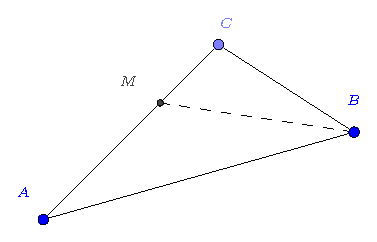
\includegraphics{../images/img007068-1}
\end{center}
}
\indication{Où se trouve le point $M$ sur le segment $[AC]$ ?}
\reponse{
Soit $D$ le symétrique de $B$ par rapport à $C$.

\begin{center}
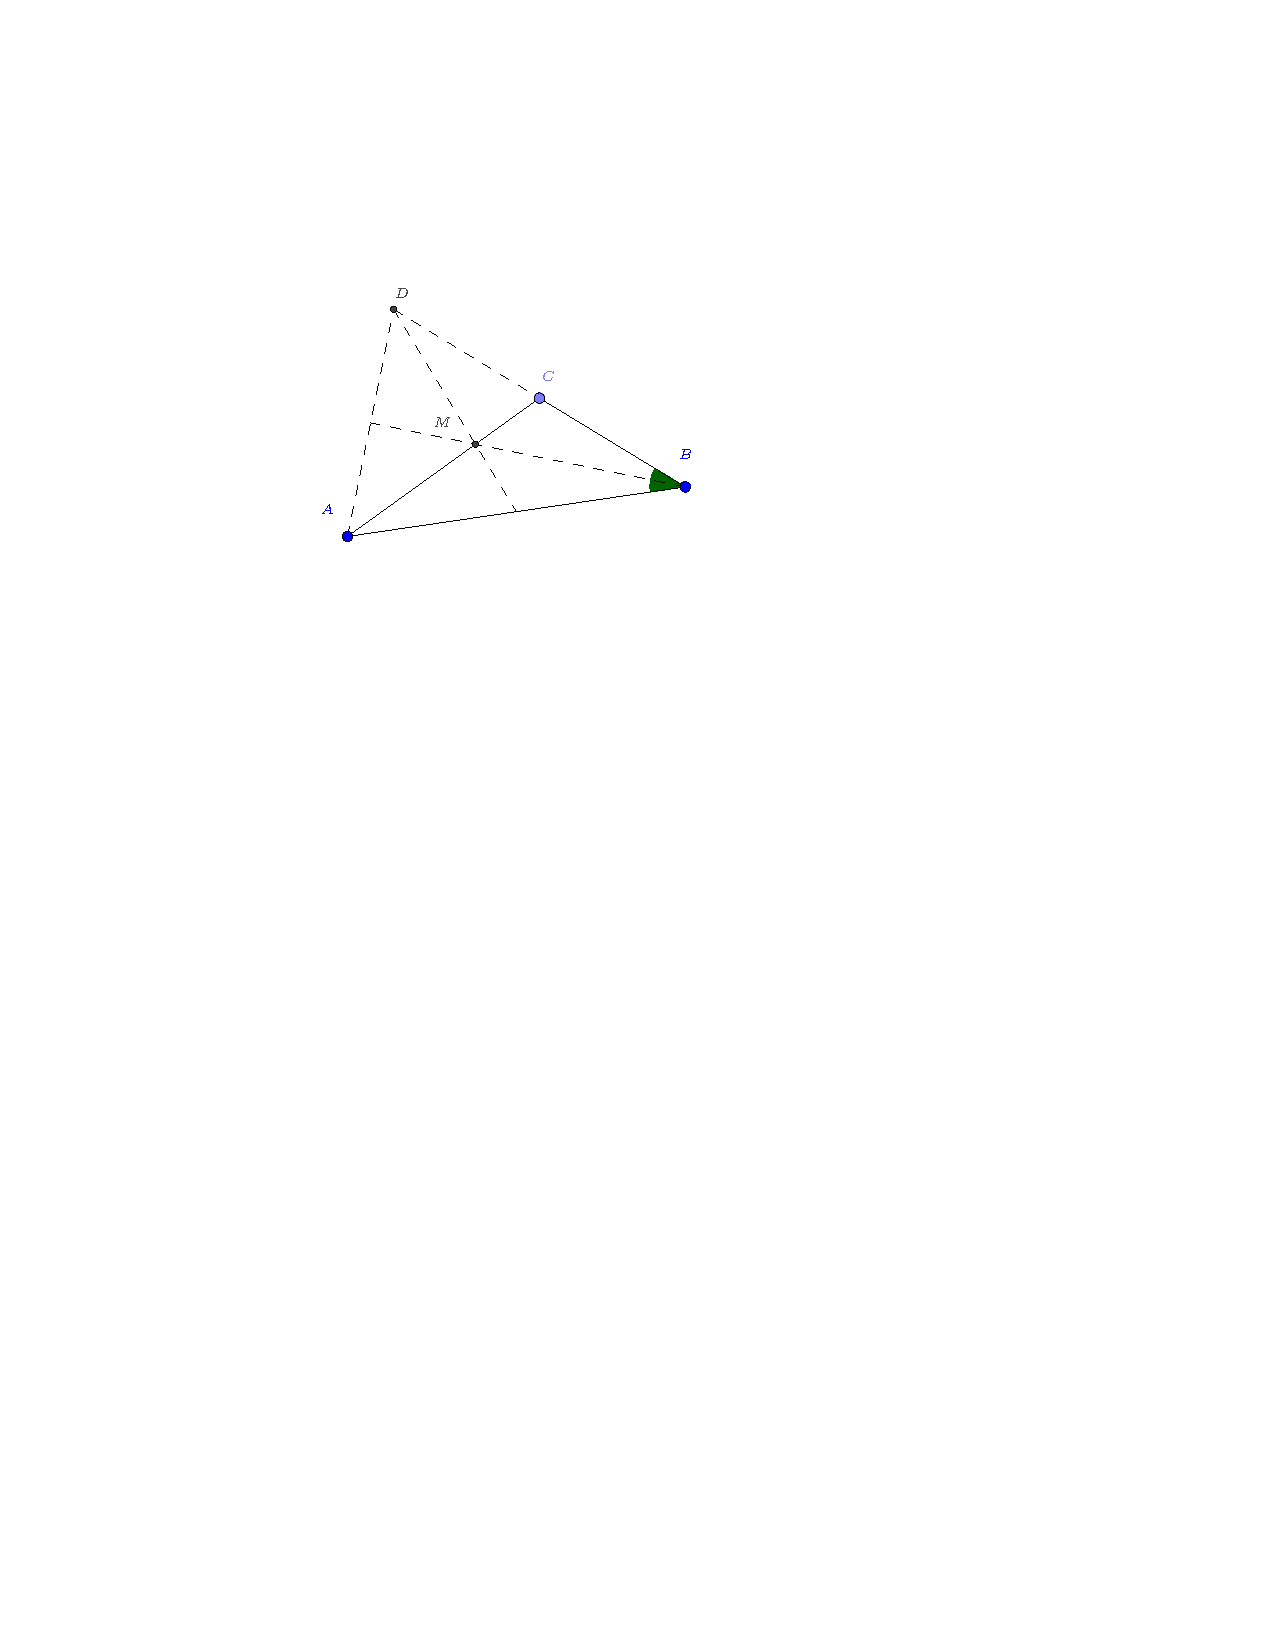
\includegraphics{../images/img007068-2}
\end{center}

Alors $[AC]$ est une médiane de $ABD$ et $M$ est son centre de gravité. Comme $BA=2BC=BD$, le triangle $ABD$ est isocèle en $B$. On en déduit que la médiane issue de $B$ est également la bissectrice issue de $B$. Les angles $\widehat{ABM}$ et $\widehat{MBC}$ sont donc égaux.
}
}
